\documentclass [7pt]{beamer}
\author{Mehrshad Adham}
\title{Example 14 \& 16}

\usepackage{xcolor}	
\usepackage{tikz}
\usepackage{textgreek}
\usetheme{Frankfurt}
\useoutertheme{infolines}
\usepackage{ragged2e}
\usepackage{amsmath}
\usepackage{amssymb}
\pgfdeclarelayer{nodelayer}
\pgfdeclarelayer{edgelayer}
\pgfsetlayers{edgelayer,nodelayer,main}
\tikzset{newstyle/.style={thick}}
\tikzset{simple/.style={thick}}
\tikzstyle{new style}=[fill=white, draw=black, shape=circle, scale=1]
\tikzstyle{none}=[fill=none, draw=none, shape=circle, scale=0]
\tikzstyle{new style 0}=[fill=white, draw=black, shape=circle, scale=0.75]
\tikzstyle{new edge style 0}=[draw=black, ->]
\date{}
\begin{document}
\small
\section*{Example NO. 14\&16 }
\subsection*{Mehrshad Adham }	
\begin{frame}
\justifying	
 14. Construct a regular grammar for the RE, L = (a + b)*(aa + bb)(a + b)*.
 \hspace*{0.5cm}	  		 \textit{\textbf{Solution:}} The NFA for the RE is
\begin{center}
    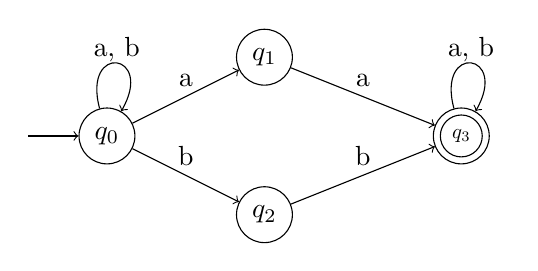
\begin{tikzpicture}
	\begin{pgfonlayer}{nodelayer}
		\node [style=new style] (0) at (-2, 0) {$q_0$};
		\node [style=new style] (1) at (2.5, 0) {$q_3$};
		\node [style=new style] (2) at (0, -1) {$q_2$};
		\node [style=new style] (3) at (0, 1) {$q_1$};
		\node [style=new style 0] (4) at (2.5, 0) {$q_3$};
		\node [style=none] (5) at (-3, 0) {};
	\end{pgfonlayer}
	\begin{pgfonlayer}{edgelayer}
		\draw [style=new edge style 0] (5.center) to (0);
		\draw [style=new edge style 0] (0) to node [above=0pt] {a} (3);
		\draw [style=new edge style 0] (0) to node [above=0pt] {b} (2);
		\draw [style=new edge style 0, in=60, out=105, loop] (0) to node [above=-3pt] {a, b} ();
		\draw [style=new edge style 0, in=60, out=105, loop] (1) to node [above=-3pt] {a, b} ();
		\draw [style=new edge style 0] (3) to node [above=0pt] {a} (1);
		\draw [style=new edge style 0] (2) to node [above=0pt] {b} (1);
	\end{pgfonlayer}
\end{tikzpicture}
\end{center}
There are four states in the FA. So, in the regular grammar, there are four non-terminals.
 Let us take them as A (for q\textsubscript{0}), B (for q\textsubscript{1}), C (for q\textsubscript{2}), and D (for q\textsubscript{3}).\\Now, we have to construct the production rules of the grammar.\\For the state q\textsubscript{0}, the production rules are\\ \hspace*{3cm} A → aA, A → bA, A → aB, A → bC.\\For the state q\textsubscript{1}, the production rules are\\ \hspace*{3cm} B → aD, B → a (as D is the final state).\\ For the state q\textsubscript{2}, the production rules are\\ \hspace*{3cm} C → b D, C → b (as D is the final state).
\end{frame}
\begin{frame}
\justifying	
For the state q\textsubscript{3}, the production rules are\\ \hspace*{3cm} D → aD, D → bD, D → a/ b.\\The grammar = \{V\textsubscript{N}, Σ, P, S\}\\ \hspace*{3cm}V\textsubscript{N} = {A, B, C, D} Σ = {a, b}\\
 \hspace*{3cm}P : A → aA/bA/aB/bC\\
 \hspace*{3cm}B → aD/a\\
 \hspace*{3cm}C → bD/b\\
 \hspace*{3cm}D → aD/bD/a/b.\\
16. Find the RE recognized by the finite state automaton of the following figure. [GATE 1994]
\begin{center}
    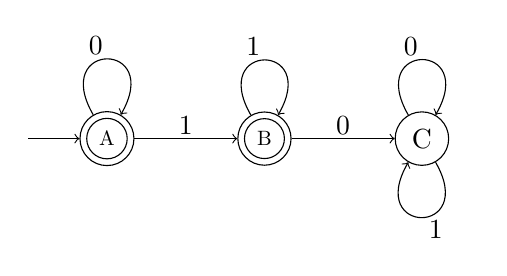
\begin{tikzpicture}
	\begin{pgfonlayer}{nodelayer}
		\node [style=new style] (0) at (-2, 0) {A};
		\node [style=new style] (1) at (0, 0) {B};
		\node [style=new style] (2) at (2, 0) {C};
		\node [style=none] (3) at (-3, 0) {};
		\node [style=new style 0] (4) at (-2, 0) {A};
		\node [style=new style 0] (5) at (0, 0) {B};
	\end{pgfonlayer}
	\begin{pgfonlayer}{edgelayer}
		\draw [style=new edge style 0] (0) to node [above=-2pt] {1} (1);
		\draw [style=new edge style 0] (1) to node [above=-2pt] {0} (2);
		\draw [style=new edge style 0] (3.center) to (0);
		\draw [style=new edge style 0, in=-120, out=-60, loop] (2) to node [above left=-11pt] {1} ();
		\draw [style=new edge style 0, in=60, out=120, loop] (2) to node [above left=-2pt] {0} ();
		\draw [style=new edge style 0, in=60, out=120, loop] (0) to node [above left=-2pt] {0} ();
		\draw [style=new edge style 0, in=60, out=120, loop] (1) to node [above left=-2pt] {1} ();
	\end{pgfonlayer}
\end{tikzpicture}
\end{center}
\end{frame}
\begin{frame}
\justifying
\textit{\textbf{Solution:}} The equation for the FA is\\
\hspace*{5cm} A = 0A + $\land$ \hspace*{4.5cm}(1)\\
\hspace*{5cm} B = 1A + 1B \hspace*{4.3cm}(2)\\
\hspace*{5cm} C = 0B + 0C + 1C \hspace*{3.5cm}(3)\\
Solving the equation (1) using the Arden’s theorem, we get A = $\land$0* = 0*.\\
 Putting the value of A in equation (2), we get\\
\hspace*{5cm} B = 10* + 1B.\\
 Using the Arden’s theorem, we get\\
\hspace*{5cm} B = 10*1*.\\
 Both A and B are final states, and thus the string accepted by the FA is\\
\hspace*{5cm} 0* + 10*1*\\
\hspace*{5cm}= 0* ($\land$ + 11*) = 0*1* (as $\land$ + RR* = R*).
\end{frame}

\end{document}